\chapter{Zeeman Effect}
%************************************************
\begin{flushright}
October 21 to November 4, 2013 \\
\end{flushright}

\section{Introduction}

We start with a classical description of the Zeeman Splitting and
Polarization, beginning with justifying how we can model the Atom
as a harmonic oscillator. Next, we'll discuss the Fabry Parot device
and its basics. We'll then go on to discuss how it operates to produce
fringes in various setups. We then briefly mention the constant deviation
spectrometer and finally, discuss the setup of the two related experiments.


\section{Classical Description of Zeeman Splitting}


\subsection{Modeling the Atom as a harmonic oscillator}

Consider a simple atomic system with a heavy nucleus and a light electron.
In the rest frame of the electron, at equilibrium we can write

\[
m_{e}a_{0}=0=\frac{m_{e}v^{2}}{r_{0}}-\frac{kq^{2}}{r_{0}^{2}}
\]
where radially inwards direction has been taken as negative and $r_{0}$
is the radius of the orbit. However, if we displace the the electron
from its equilibrium trajectory, and assume the velocity remains unchanged,
we can write

\[
m_{e}a=\frac{m_{e}v^{2}}{r_{0}+r}-\frac{kq^{2}}{\left(r_{0}+r\right)^{2}}
\]
We can now taylor expand both the force term and the pseudo force
to obtain

\[
m_{e}a=m_{e}v^{2}\left(\frac{1}{r_{0}}-\frac{r}{r_{0}^{2}}+\frac{r^{2}}{r_{0}^{3}}+\ldots\right)-kq^{2}\left(\frac{1}{r_{0}^{2}}-\frac{2r}{r_{0}^{3}}+\frac{3r^{2}}{r_{0}^{4}}+\ldots\right)
\]
where $r$ is the perturbation from the equilibrium point (radially
outward corresponds to $r>0$). Keeping only leading order terms and
applying the equilibrium relation, we get

\[
m_{e}a=\left(-\frac{mv^{2}}{r_{0}}+\frac{2kq^{2}}{r_{0}^{3}}\right)r=-m\omega_{0}^{2}r
\]
where we have 
\[
\omega_{0}^{2}\equiv\left(\frac{v^{2}}{r_{0}}-\frac{2kq^{2}}{mr_{0}^{3}}\right)
\]
Although we haven't shown $\omega_{0}$ to be real, we assume it to
be so. This explains why we can model to first order, a simple (hydrogen)
atom, as a harmonic oscillator.


\subsection{Zeeman Splitting and Polarization}

It is established now that an atom in a magnetic field can be modelled
as a simple harmonic oscillator. Let $\omega_{o}$ be the frequency
of motion in the absence of magnetic field; the electron has the same
resonant frequency in motion along $x$, $y$ and $z$ directions.
In the presence of magnetic field B, the equation of motion, in the
rest frame of electron is given as 
\[
m_{o}\frac{dv}{dt}=-m_{o}\omega_{o}^{2}r-ev\times B
\]
where the $r$ is the position vector and $v=\dot{r}$ is the velocity
vector. If the direction of the field is along the $z$ axis, $B=B\hat{e}_{z}$

\[
\ddot{r}+2\Omega_{L}\dot{r}\times\hat{e}_{z}+\omega_{o}^{2}r=0
\]
 where $\Omega_{L}$ is the Larmor frequency defined as
\[
\Omega_{L}=\frac{eB}{2m_{o}}
\]
 Applying the matrix method to solve the above equation, we look for
a solution in the form of a vector oscillating at $\omega$ such as
\[
r=Re\left\{ \left(\begin{array}{c}
x\\
y\\
z
\end{array}\right)exp(-i\omega t)\right\} 
\]
 and obtain the following matrix
\[
\left(\begin{array}{ccc}
\omega_{o}^{2} & -2i\omega\Omega_{L} & 0\\
2i\omega\Omega_{L} & \omega_{o}^{2} & 0\\
0 & 0 & \omega_{o}^{2}
\end{array}\right)\left(\begin{array}{c}
x\\
y\\
z
\end{array}\right)=\omega^{2}\left(\begin{array}{c}
x\\
y\\
z
\end{array}\right)
\]
 we then find the eigen values by building the following determinant
\[
\left|\begin{array}{ccc}
\omega_{o}^{2}-\omega^{2} & -2i\omega\Omega_{L} & 0\\
2i\omega\Omega_{L} & \omega_{o}^{2}-\omega^{2} & 0\\
0 & 0 & \omega_{o}^{2}-\omega^{2}
\end{array}\right|=0
\]
 which then gives 
\[
\left\{ \omega^{4}-\left(2\omega_{o}^{2}+4\Omega_{L}^{2}\right)\omega^{2}+\omega_{o}^{2}\right\} \left(\omega^{2}-\omega_{o}^{2}\right)=0
\]
By inspection, $\omega=\omega_{o}$is one solution. For $\Omega_{L}\ll\omega_{o}$
, the approximate frequencies are $\omega\approx\omega_{o}\pm\Omega_{L}$.
The eigen vectors corresponding to these
\[
r=\left(\begin{array}{c}
cos(\omega_{o}-\Omega_{L})t\\
-sin(\omega_{o}-\Omega_{L})t\\
0
\end{array}\right),\left(\begin{array}{c}
0\\
0\\
cos(\omega_{o}t)
\end{array}\right),\left(\begin{array}{c}
cos(\omega_{o}+\Omega_{L})t\\
sin(\omega_{o}+\Omega_{L})t\\
0
\end{array}\right)
\]
 the motion along $z$ axis is not affected by the magnetic field
and the angular frequency remains $\omega_{o}$. The off diagonal
terms $\pm2i\omega\Omega_{L}$of the matrix depict the coupling of
the motions in the $x$ and $y$ directions resulting in circular
motion confined to the $xy$ plane, with frequencies shifted from
the Larmor frequency $\omega_{o}$. Evidently the applied external
field separates the initially equal frequencies.

The direction of radiation is given by the $a\times r$, where the
$a$ is the acceleration and $r$ is the position vector of the electron. 

The electron oscillating parallel to $B$ radiates with angular frequency
$\omega_{o}$, in the $y$ direction when seen in the $xy$ plane,
and no radiation is observed in the direction of the magnetic field.

The circular motion of the electron produces radiation with angular
frequencies $\omega_{o}+\Omega_{L}$ and $\omega_{o}-\Omega_{L}$.
Looking edge-on, this circular motion is seen as a linear sinusoidal
motion. Seeing along the $y$ axis, the linear motion is along the
$x$ axis, and the radiation is polarised perpendicular to the magnetic
field. Looking along the $z$ direction, the motion is circular and
the radiation is circularly polarised, associated with the respective
frequencies.


\subsection{Limitations}

Other than the inconsistencies of the assumptions, the fact that we
need a discharge tube for observing the effect is not explained. For
the purposes of this experiment, postponing the precise quantum mechanical
description for later, I would just state that radiation we observe
is when the electron jumps down an `orbit'. This essentially means
that two given `orbit' is split and due to selection rules, we see
only three wavelengths of radiation, shifted up, shifted down and
the original (before application of the magnetic field).

Another peculiar result seems to be that the eigenvector passes through
the centre of the atom! This is a sort of projection, or so we were
told. We weren't able to identify the source of this error.


\section{Fabry Parot}

This is a very elegant device. This harnesses a principle very similar
to that of the interferometer. Instead of explaining in words, let's
derive it straight away. Consider
a ray incident on the etalon at an angel $\theta$ with respect to
the outward normal of the first surface. The corresponding virtual ray
(with respect to the second surface) can be constructed a distance
$2d$ behind the real ray. Considering that the distance between the
screen and the etalon, $D\gg d$, to see interference we simply need
to consider the path difference between these two rays, along a plane
whose normal coincides with the ray. As shown in the diagram, it follows
this distance is 
\[
\Delta\lambda=2d\cos\theta
\]
This now has very interesting repercussion. If you have a monochromatic
point source incident, depending on the angle of a ray with the normal
of the etalon surface, you would get a path difference. This results
in the formation of circular fringes with constructive interference
happening on specific radii (explicit calculations have been done
in the next experiment). If there was another monochromatic source
at the same location, you would again get a circular pattern corresponding
to the new wavelength. Keep this in mind. We'll use this property
often.


\subsection{The effect of sources and lenses}

It is important to understand in some detail what happens under the
permutation of the following conditions
\begin{enumerate}
\item Monochromatic Source

\begin{enumerate}
\item Point
\item Extended
\end{enumerate}
\item Lens

\begin{enumerate}
\item Before (the source is on the focal plane)
\item After (if you remove the lens and look directly, it is equivalent,
the eye has a lens)
\end{enumerate}
\item {[}not discussed{]} Eye after lens
\end{enumerate}
So there will be $2^{3}=8$ possibilities. Let's do them all. Consider
a Monochromatic:
\begin{enumerate}
\item Point Source, without any lens\\
This was discussed earlier in this section. The result is \emph{circular
fringes}.
\item Extended Source, without any lens\\
The point source and the etalon can be effectively treated as two
point sources, $2d$ distance apart ($d$ is as usual, the distance
between the mirrors of the etalon). Using superposition, we can claim
the pattern should be a superposition of multiple circular fringes,
corresponding to everypoint of the source. Effectively, \emph{no pattern}
should be visible.
\item Point Source, with a lens before, but none after\\
The result is that all the light rays incident on the etalon would
be parallel. Thus a uniform intensity pattern should be obtained,
and changing the angle of the etalon with respect to the principle
axis of the lens ($\theta$) should yield \emph{different uniform
intensities}.
\item Extended Source, with a lens before, but none after\\
In this case, each point on the extended source is mapped to a parallel
light beam of a fixed angle $\theta$ with respect to the principle
axis, as a function of its (the point's) distance from the principle
axis. The etalon will simply add a phase difference of $2d\cos\theta$
to a beam of a given orientation. Since there's no lens after, all
these will fall on a screen and result in a \emph{uniform intensity,
independent of the orientation of the etalon}.
\item Point Source, with a lens before and a lens after\\
The image obtained will be that of a \emph{single point}, except it
would be either bright or dark, \emph{depending on the orientation}
of the etalon ($\theta$).
\item Extended Source, with a lens before and a lens after\\
The analysis from the previous part follows. The other lens focusses
parallel beams on different points on the focal plane, essentially
mapping $\theta$ to position. Since the phase difference depended
on angle $\theta$, thus different points on the screen would be bright
or dark, depending on its value. Symmetry considerations immediately
tell us that the pattern will be \emph{circular fringes} (may be cropped
though, depending on the shape of the extended source). \\
{[}`Prism' zeeman like{]}
\item Point Source, without a lens before, but with a lens after\\
This is perhaps the most non-trivial case. Again, we effectively have
two point sources, but they are followed by a lens (both points are
farther away from $2F$). Using the limiting size case, one can find
the resultant position of the image for both points. Now the problem
has been significantly been simplified. Given some position of the
screen (taken to be the focal plane of the lens here), for any given
point on the screen, we construct two lines (representing the rays);
the first joining the first point's image and the screen point and
the second joining the second point's image and the screen point.
Extending this line, we can find the point of intersection with the
lens. Now we connect the intersection of the first line with the lens,
with a line to the first source point. Similarly for the second point
we repeat the procedure. Using this, one can calculate the path difference
between the two rays that superpose on the screen. Without quantifying,
from the symmetry, it is clear that a \emph{circular pattern} will
again be obtained in this case. \\
{[}`TV' Zeeman like if you consider the source to be a point source{]}
\item Extended Source, without a lens before, but with a lens after\\
Here again, a \emph{circular pattern} is obtained. This can be easily
understood again by considering two extended sources. Now we consider
only parallel beams coming from the corresponding points of the two
sources, for other beams (non parallel) will either not be focussed
or (different points, but parallel) not coherent. As earlier, the
etalon will add a phase difference depending on the angle $\theta$,
and the lens will converge at a location, depending again on $\theta$.
Thus, we get the aforesaid pattern. \\
{[}Michelson, `TV' Zeeman like{]}
\end{enumerate}
Note however that if the object is placed between $F$ and $2F$ (where
$F$ is the focal point of the lens) then one can simply substitute
the source to be placed at the point where the image will be formed,
had a screen been placed there; then the setup can be matched to the
possibilities given above and proceed accordingly. Further, in case
of a point source along the principle axis, we can find the image
position by first finding the same for an extended source and then
take its size limit to zero.


\section{Constant Deviation Spectrometer}

In a usual spectrometer, the wavelength resolved beam is not parallel.
This uses a prism as shown in the diagram in the last section. This prism
produces a parallel resolved beam. The details haven't been worked
out for this part of the apparatus wasn't used for calculations.


\section{The Setup}


\subsection{The `TV' Zeeman (polarization)}

The setup consists of an electromagnet (\autoref{e4tv}), built with two coils and a
mercury cadmium lamp placed in the centre. The light can be seen through
the axis of the coils as well as through a direction perpendicular
to it. This assembly is mounted on a rotatable, well, mount. Adjacent
to the mount, there's an optical bench. The bench has a lens that
results (eventually) in a diverging beam. This is followed by the
all glorious etalon. Then we have two polarisers which are then viewed
through a magnifier on the screen using a camera.

Let us now understand what is happening. We start without polarisers.
This is the same as an extended source without a lens before (the
object is not at the focus of the lens) and a lens after. However,
the source is not monochromatic, instead it has three wavelengths.
Their circular patterns superimpose. Further, as explained in the
earlier sections, the different frequencies are polarized differently.
The polarized can be inserted to block lights of specific frequencies
and the fringe pattern correspoding to that wavelength dissapears;
resulting in a higher contrast pattern.


\subsection{The `Prism' Zeeman (splitting)}

The setup consists of collimator (\autoref{e4prism}), a special constant deviation prism,
and a telescope. The collimator has an adjustable slit width. Incident
to this can either be a sodium or mercury lamp, or a Neon discharge
tube, placed between two coils of an electromagnet. 

Let us look at what is happening. The setup starts with converting
the incident light into the shape of the slit. Then this light is
passed through the collimator. The collimator is focussed such that
the point source is in its focal plane (this is leading to a type
6 setup). This is then incident on the prism, which does two things.
It guides the light into the telescope; and it spatially displaces
different wavelengths. So effectively, the different frequencies have
become spatially displaced sources. Since the shape of the extended
source is a slit, introduction of an etalon results in the creation
of slits in the line (instead of the circular fringes). Upon application
of the magnetic field, a single frequency splits into three, and so
does the corresponding pattern. What remains to show is that this
splitting distance is directly proportional to the applied magnetic
field, and that was the experiment we performed.

%%%%%%%%%%%%%%%%%%%%%%%%%%%%%%%%%%%%
%DONT REMOVE ME
%%%%%%%%%%%%%%%%%%%%%%%%%%%%%%%%%%%%%
The observations are given in \autoref{zeemanReading} where the column names are self explanatory, the calibration of the current and magnetic field are given in \autoref{zeemanCalibration}, while the corresponding graphs are \autoref{e4z1} and \autoref{e4z2}.
\lstinputlisting{gfx/zeemanReading}\label{zeemanReading}
\lstinputlisting{gfx/zeemanCalibration}\label{zeemanCalibration}

\begin{figure}[bth]
	\begin{center}
		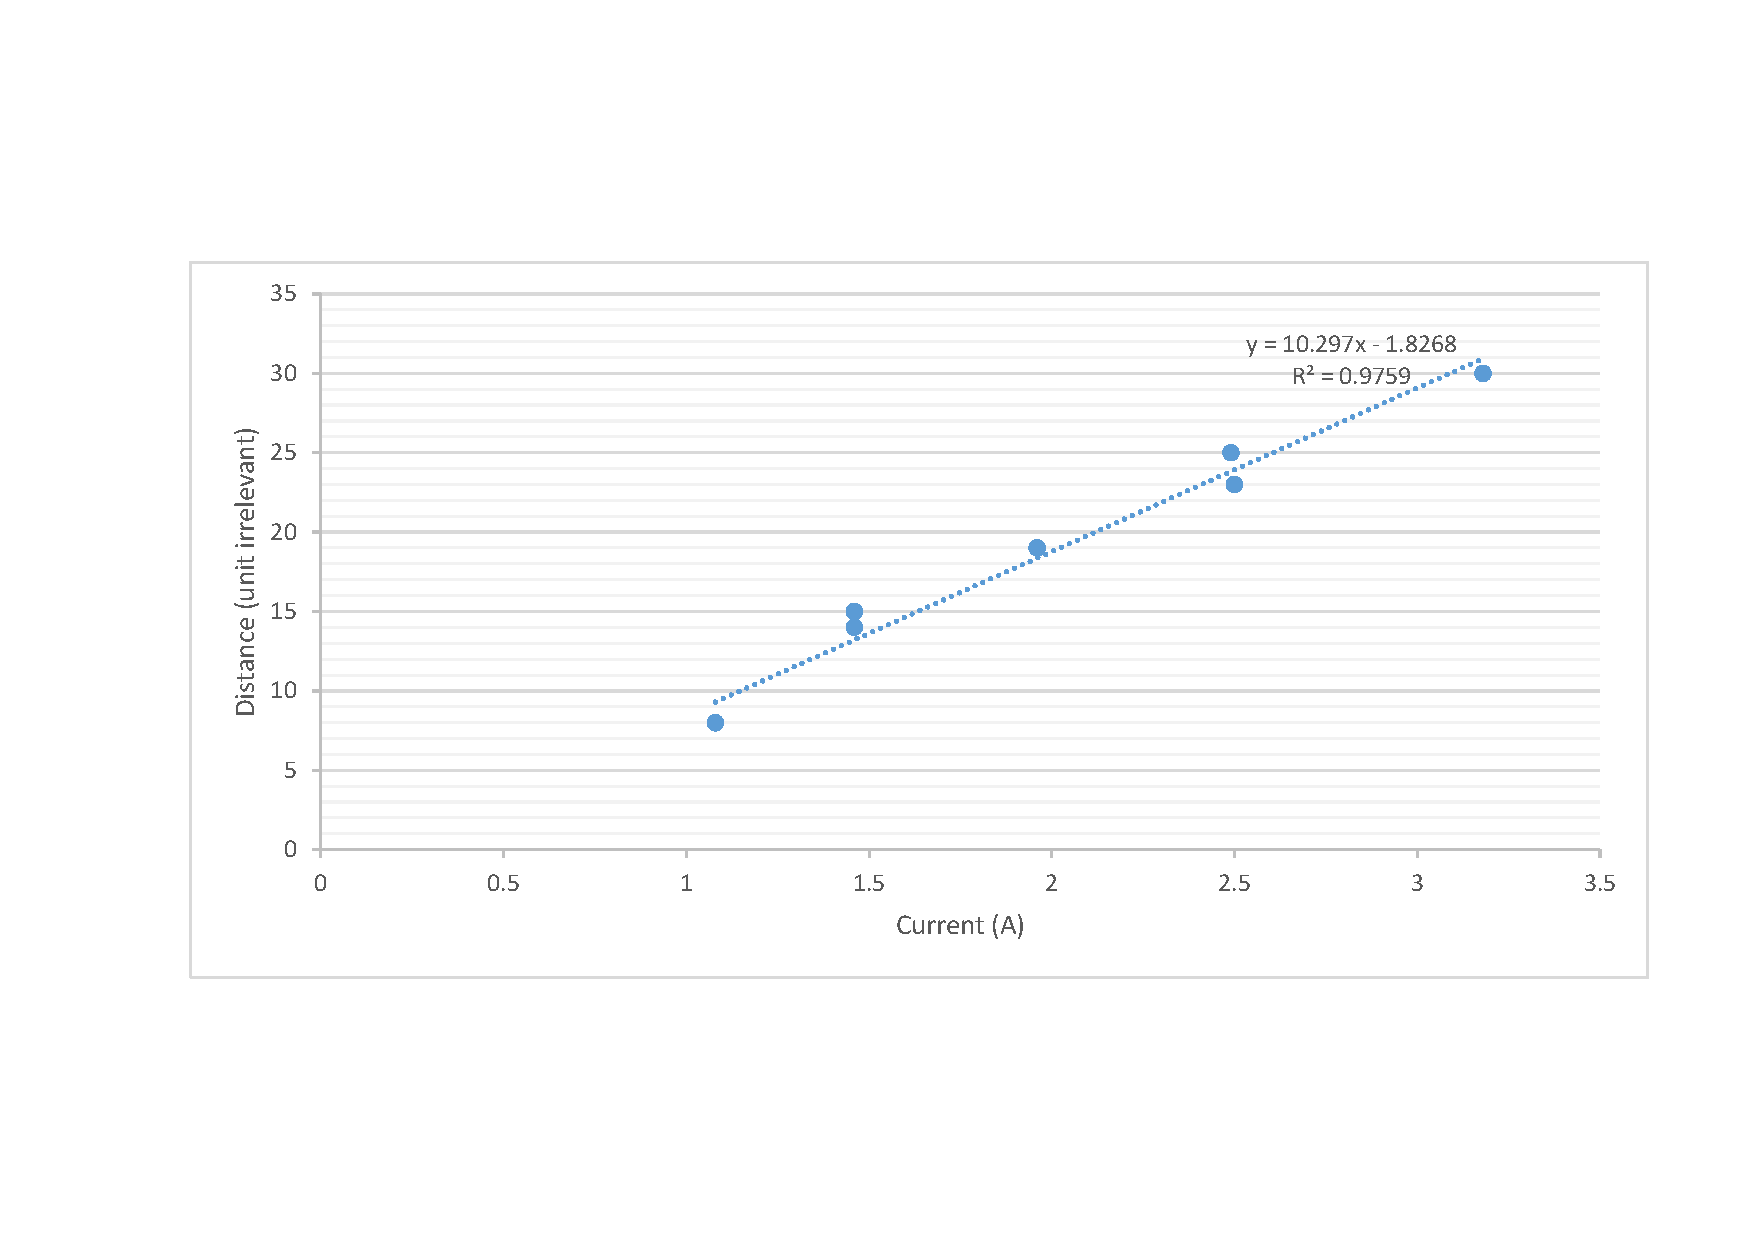
\includegraphics[width=1.3\linewidth]{gfx/4_zeeman}
	\end{center}
\caption[Split Distance vs Current]{Split Distance vs Current}
\label{e4z1}
\end{figure}

\begin{figure}[bth]
	\begin{center}
		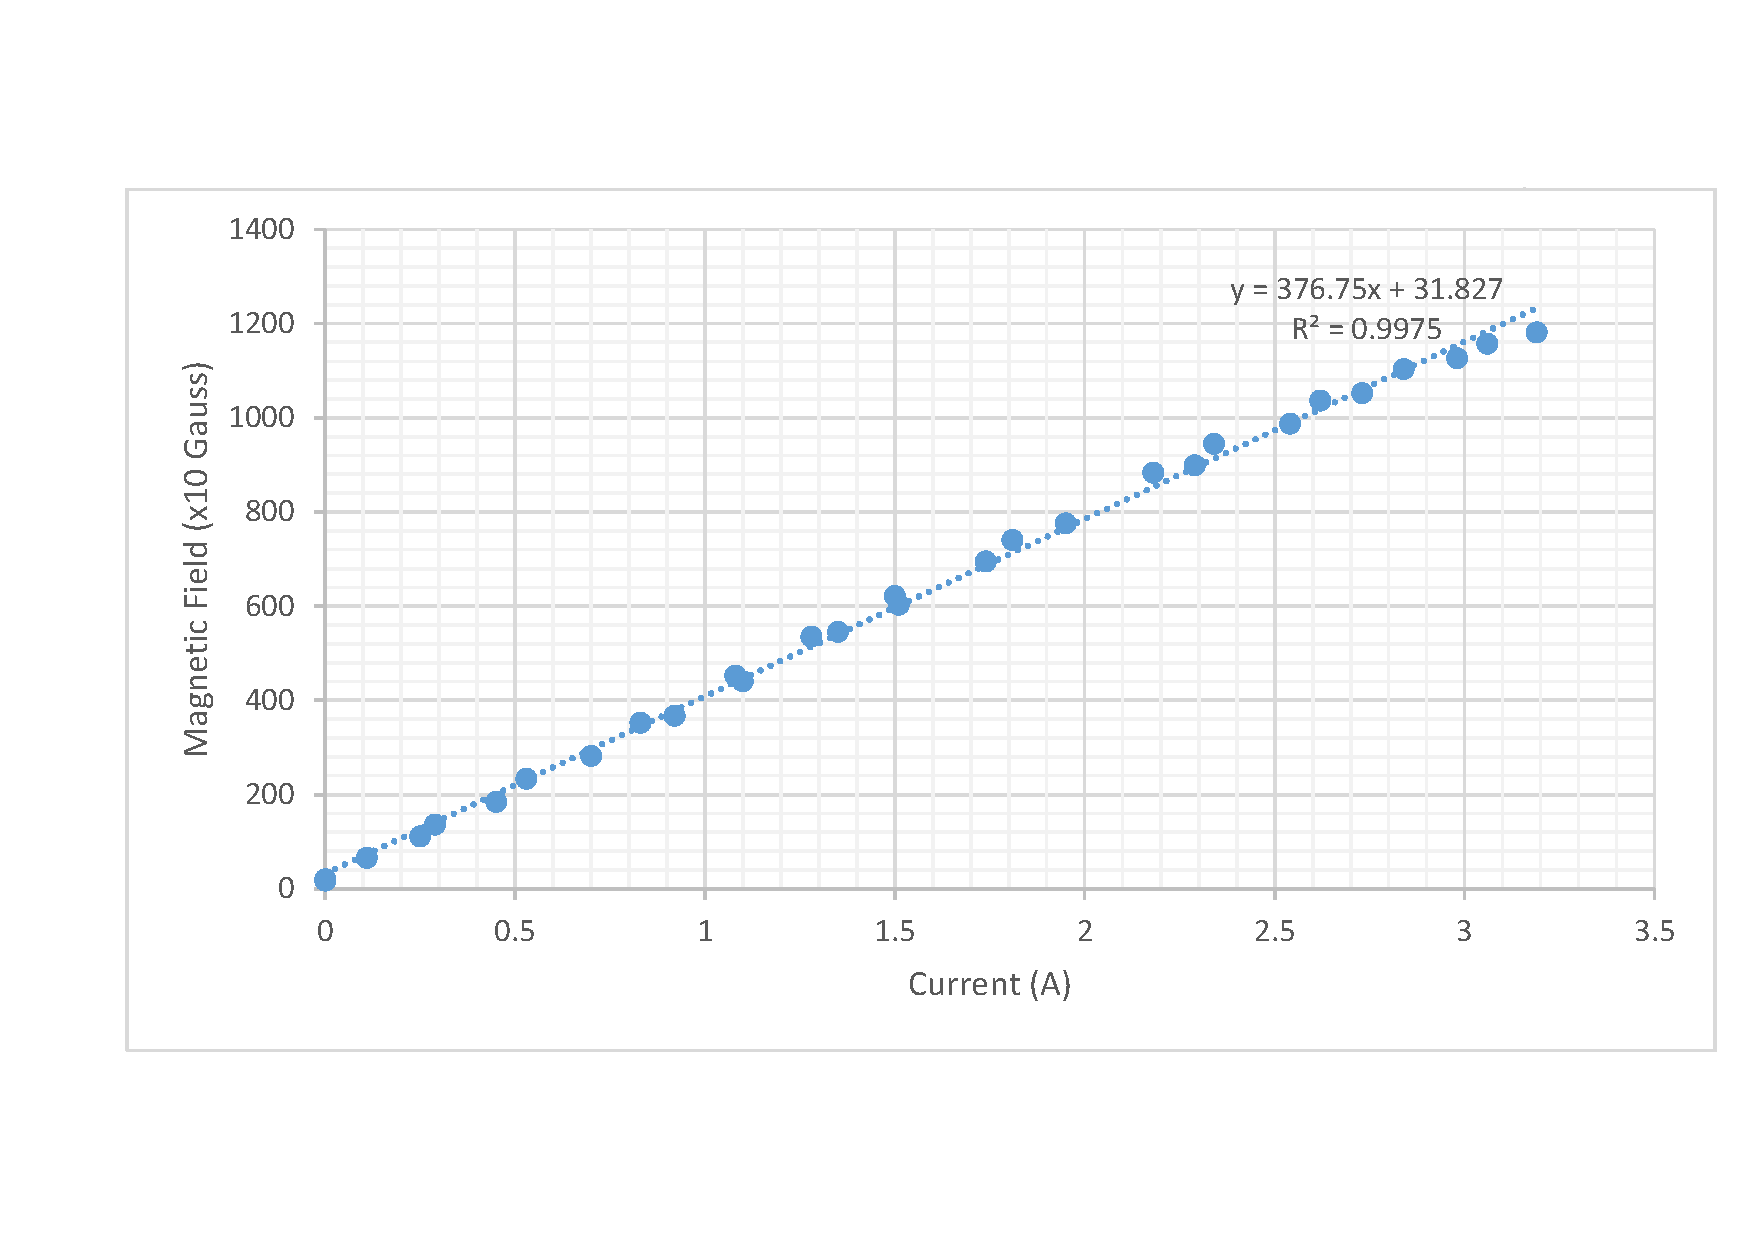
\includegraphics[width=1.3\linewidth]{gfx/4_zeemanCalibration}
	\end{center}
\caption[Calibration of Magnetic Field and Current]{Calibration of Magnetic Field and Current}
\label{e4z2}
\end{figure}

\begin{figure}[bth]
	\begin{center}
		
\includegraphics[width=1.1\linewidth]{gfx/e4_zeemanPrism}
	\end{center}
\caption[`Prism' Zeeman Setup]{`Prism' Zeeman Setup}
\label{e4prism}
\end{figure}

\begin{figure}[bth]
	\begin{center}
		
\includegraphics[width=1.0\linewidth]{gfx/e4_zeemanTV}
	\end{center}
\caption[`TV' Zeeman Setup]{`TV' Zeeman Setup}
\label{e4tv}
\end{figure}